\documentclass{ximera}

\newcommand{\RR}{\mathbb R}
\renewcommand{\d}{\,d}
\newcommand{\dd}[2][]{\frac{d #1}{d #2}}
\renewcommand{\l}{\ell}
\newcommand{\ddx}{\frac{d}{dx}}
\newcommand{\dfn}{\textbf}
\newcommand{\eval}[1]{\bigg[ #1 \bigg]}


\author{Jim Talamo}
\license{Creative Commons 3.0 By-bC}


\outcome{}


\begin{document}
\begin{exercise}
There is an important fact for the Ratio Test:

Let $p(x)$ be a polynomial.  Then:

\[
\lim_{n \to \infty} \frac{p(n+1)}{p(n)} = 1
\]

\begin{exercise}
To gain a little practice, suppose that $p(x) = x^5$.  Then the limit to evaluate is:

\[
\lim_{n \to \infty} \frac{p(n+1)}{p(n)} = \answer{\frac{(n+1)^5}{n^5}}
\]
The numerator is a polynomial of degree $\answer{5}$, and the coefficient of the $n^5$ term is $\answer{1}$.

The denominator is a polynomial of degree $\answer{5}$, and the coefficient of the $n^5$ term is $\answer{1}$.

Hence, the limit is $\answer{1}$.

\begin{exercise}
To explore this a little more, now set $p(x) = x^5+4x^3+7$.  Then:
\[
\lim_{n \to \infty} \frac{p(n+1)}{p(n)} = \answer{\frac{(n+1)^5+4(n+1)^3+7}{n^5+4n^3+7}}
\]

Note that $(n+1)^5$ is a polynomial of degree $\answer{5}$, $(n+1)^3$ is a polynomial of degree $\answer{3}$, so without expanding any of these powers out, the numerator is a polynomial of degree $\answer{5}$, and the coefficient of the $n^5$ term is $\answer{1}$.

The denominator is a polynomial of degree $\answer{5}$, and the coefficient of the $n^5$ term is $\answer{1}$.

Hence, the limit is $\answer{1}$.

\end{exercise}


\begin{exercise}
One of the major consequences of this is that multiplying or dividing a given \emph{sequence} by a polynomial will not affect the limit required in the Ratio Test.  Indeed, consider the series $\sum_{k=1}^{\infty} \frac{1}{2^k}$.  Note that this is a geometric series, but we could establish its convergence using the Ratio Test.  Indeed, here:

\[
L = \lim_{n \to \infty} \frac{a_{n+1}}{a_n} = \lim_{n \to \infty} \frac{1}{2^{n+1}}\cdot 2^n = \answer{\frac{1}{2}}
\]

Now, let's multiply the original sequence defined by the rule $a_n = \left(\frac{1}{2}\right)^n$ by the polynomial $p(n) = n^5$ and try to sum its terms.  That is, we want to consider the series $\sum_{k=1}^{\infty} \frac{k^5}{2^k}$. We find:

\[
L =  \lim_{n \to \infty} \frac{(n+1)^5}{2^{n+1}} \cdot \frac{2^n}{n^5} =  \lim_{n \to \infty} \frac{2^n}{2^{n+1}} \cdot \frac{(n+1)^5}{n^5} =  \answer{\frac{1}{2}} \cdot \answer{1}
\]

Introducing the $n^5$ term into the numerator did not affect the value of $L$.

Indeed, for the series $\sum_{k=1}^{\infty} \frac{1}{2^k}$, we found that $L=\answer{\frac{1}{2}}$ and for the series $\sum_{k=1}^{\infty} \frac{k^5}{2^k}$, we found $L=\answer{\frac{1}{2}}$. 

\begin{exercise}
One of the major consequences of this now is that a series must have a term that grows at least exponentially in order for the Ratio Test to have a chance to be conclusive!  More explicitly, let $p, q > 0$, $a>1$, and consider the growth rates results for \emph{sequences}:

\begin{image}
  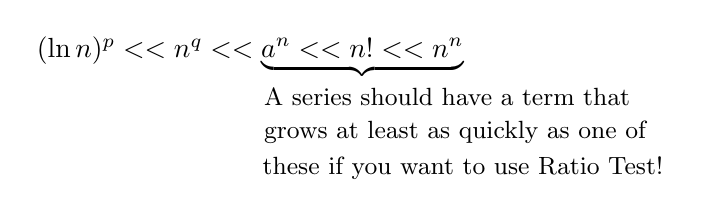
\begin{tikzpicture}
        \node at (0,0) {
          $(\ln n)^p << n^q << \underbrace{a^n << n! << n^n}$
        };
        \node at (2.5,-.5) {\small{A series should have a term that}};
         \node at (2.6,-.95) {\small{grows at least as quickly as one of}};
         \node at (2.7,-1.4) {\small{these if you want to use Ratio Test! }};
      \end{tikzpicture}
  \end{image}

For which of the following series would the Ratio Test be conclusive?  That is, which of the following would either converge or diverge as a consequence of the Ratio Test?
\begin{selectAll}
\choice{$\sum_{k=1}^{\infty} \frac{k^3+2k-1}{k^2+2}$}
\choice[correct]{$\sum_{k=1}^{\infty} \frac{\ln(k) +k^2}{k!}$}
\choice[correct]{$\sum_{k=1}^{\infty} \frac{k^{10}}{5^k}$}
\choice{$\sum_{k=1}^{\infty} \frac{(\ln k)^{80}}{k^5}$}
\choice{$\sum_{k=1}^{\infty} k^{2018}$}
\choice[correct]{$\sum_{k=1}^{\infty} \frac{2^k}{k^k}$}
\end{selectAll}

\end{exercise}
\end{exercise}
\end{exercise}
\end{exercise}
\end{document}
